\documentclass[10pt, a4paper, oneside]{article}
\usepackage[utf8]{inputenc}

% To assign English fonts
% \usepackage{fontspec}
% \setmainfont{Roboto-Regular.ttf}[
%   % Path=/Some Folder Your Fonts/ , % If you want to assign folder path which contains your font files.
%   BoldFont=Roboto-Bold.ttf ,
%   ItalicFont=Roboto-Italic.ttf ,
%   BoldItalicFont=Roboto-BoldItalic.ttf
% ]

% To assign Chinese (CJK) fonts
% \usepackage[AutoFakeBold=1, AutoFakeSlant=0.2]{xeCJK}
% \setCJKmainfont{NotoSerifTC-Regular.otf}[
%   BoldFont=NotoSerifTC-Bold.otf
% ]

\setlength\parindent{0pt}


\usepackage{geometry}
\geometry{
  left=3.0cm,
  top=2.2cm,
  right=3.0cm,
  bottom=2.5cm,
  footskip=1.0cm
}


\usepackage[colorlinks=true, allcolors=blue, unicode]{hyperref}
\usepackage{enumitem}
\providecommand{\tightlist}{%
  \setlength{\itemsep}{0pt}\setlength{\parskip}{0pt}}

\usepackage{longtable,booktabs}

\usepackage{graphicx}

\usepackage{imakeidx}
\makeindex[intoc]

\usepackage{fancyhdr}
\renewcommand{\headrulewidth}{0pt}

\renewcommand{\footrulewidth}{0.4pt}

\fancyhf{}
\pagenumbering{arabic}
\pagestyle{fancy}
\fancyfoot{}
\fancyfoot[L]{\space}
\fancyfoot[C]{\leftmark}
\fancyfoot[R]{\thepage}
\fancypagestyle{plain}{\pagestyle{fancy}}

\usepackage{puredoc-titlepage}

\usepackage{amsmath}
\usepackage{amsthm}
\usepackage{amsfonts}
\usepackage{bm}
\newtheorem{theorem}{Theorem} % Define theorem


\begin{document}
\puredocTitlepageTitle{Demo Article}
\puredocTitlepageSubtitle{Single Title Page}
\puredocTitlepageVersion{Second Edition}
%%
\puredocTitlepageAuthors{Wei-Chun Tsai}{Taiwan No. 1 Company}
\puredocTitlepageAuthors{Bae Liu}{Taiwan No. 2 Company}
%%
\puredocTitlepageDate{\today}
%%
\puredocTitlepagePublisherFig
[4.5cm]
{cambridge.png}
\puredocTitlepagePublisherInfo{Taipei, Tokyo, New York}
%%
\puredocTitlepageMaketitle[left]
\setcounter{page}{2}


{
\pagestyle{empty}
\vspace*{1cm}
\section*{\centering \emph{In memory of my brother, John Nash}}
\subsection*{\centering Risk is our business.}

{\centering \emph{You would have enjoyed it.} \par}


\subsection*{\centering Are you ready?}

{\centering \emph{Let's go!} \par}


\clearpage
}

\setcounter{tocdepth}{3}
{ \hypersetup{hidelinks} \tableofcontents } \clearpage
{ \hypersetup{hidelinks} \listoftables } \clearpage
{ \hypersetup{hidelinks} \listoffigures } \clearpage

\section{Basic Usage}\label{basic-usage}

Here we would like to show you some basic structures
including paragraphs, links, lists, verbatims (usually for code blocks),
tables, figures, footnotes, index, and bibliography.
If you want to force to make a newline, you can add an empty line or use the command \texttt{\textbackslash{}newline}.
If you want to force to start a whole new page, you can use the command \texttt{\textbackslash{}clearpage} before your new content.

\subsection{\texorpdfstring{Paragraph \label{start-paragraph}}{Paragraph }}\label{paragraph}

The following is a paragraph.

Lorem ipsum dolor sit amet, consectetur adipiscing elit.
Duis ullamcorper neque sit amet lectus facilisis sed luctus nisl iaculis.

If you use a \texttt{\textbackslash{}label\{start-paragraph\}} in the section/chapter title, then you could use a

\texttt{\textbackslash{}ref\{start-paragraph\}} to refer to this section/chapter.
For example, please refer to \ref{start-paragraph}.

\subsection{Link}\label{link}

Here is a link =\textgreater{} \href{https://www.google.com}{A link to Google}

\subsection{List}\label{list}

The following is a list.

\begin{itemize}
\tightlist
\item
  The 1st main item

  \begin{itemize}
  \tightlist
  \item
    A sub item 1 of the 1st main item
  \item
    A sub item 2 of the 1st main item
  \end{itemize}
\item
  The 2nd main item

  \begin{itemize}
  \tightlist
  \item
    A sub item 1 of the 2nd main item
  \item
    A sub item 2 of the 2nd main item
  \end{itemize}
\item
  The 3rd main item

  \begin{itemize}
  \tightlist
  \item
    A sub item 1 of the 3rd main item
  \item
    A sub item 2 of the 3rd main item
  \end{itemize}
\end{itemize}

\subsection{Verbatim}\label{verbatim}

The following is a verbatim which is usually to show a code block (use \texttt{python} as an example).

\begin{verbatim}
print 'Hello World!'

for i in [ 'Hello', 'World!' ]:
  print i

if True:
  print 'Hello World!'
else:
  print 'Stay at home.'
\end{verbatim}

\clearpage

\subsection{Table}\label{table}

\subsubsection{Standard Markdown Table}\label{standard-markdown-table}

A standard markdown table supports single line only in each column and its width can not be modified.
This table can also be rendered well on common markdown platforms (ex: \href{https://github.com/}{GitHub}).

\begin{longtable}[c]{@{}rllc@{}}
\caption{A Standard Markdown Table \label{sm-table}}\tabularnewline
\toprule
Right & Left & Default & Center\tabularnewline
\midrule
\endfirsthead
\toprule
Right & Left & Default & Center\tabularnewline
\midrule
\endhead
12 & 12 & 12 & 12\tabularnewline
123 & 123 & 123 & 123\tabularnewline
1 & 1 & 1 & 1\tabularnewline
\bottomrule
\end{longtable}

If you use a \texttt{\textbackslash{}label\{sm-table\}} in the table caption, then you could use a

\texttt{\textbackslash{}ref\{sm-table\}} to refer to this table.
For example, please refer to Table. \ref{sm-table}.

\subsubsection{Extended Markdown Table}\label{extended-markdown-table}

An extended markdown table supports multiple lines in each column.
This table can \textbf{not} be rendered well on common markdown platforms (ex: \href{https://github.com/}{GitHub}).

\begin{longtable}[c]{@{}clr@{}}
\caption{An Extended Markdown Table \label{em-table}}\tabularnewline
\toprule
\begin{minipage}[b]{0.14\columnwidth}\centering\strut
Centered
Header
\strut\end{minipage} & \begin{minipage}[b]{0.11\columnwidth}\raggedright\strut
Default
Aligned
\strut\end{minipage} & \begin{minipage}[b]{0.11\columnwidth}\raggedleft\strut
Right
Aligned
\strut\end{minipage}\tabularnewline
\midrule
\endfirsthead
\toprule
\begin{minipage}[b]{0.14\columnwidth}\centering\strut
Centered
Header
\strut\end{minipage} & \begin{minipage}[b]{0.11\columnwidth}\raggedright\strut
Default
Aligned
\strut\end{minipage} & \begin{minipage}[b]{0.11\columnwidth}\raggedleft\strut
Right
Aligned
\strut\end{minipage}\tabularnewline
\midrule
\endhead
\begin{minipage}[t]{0.14\columnwidth}\centering\strut
First
\strut\end{minipage} & \begin{minipage}[t]{0.11\columnwidth}\raggedright\strut
row,
long
content
\strut\end{minipage} & \begin{minipage}[t]{0.11\columnwidth}\raggedleft\strut
12.0
\strut\end{minipage}\tabularnewline
\begin{minipage}[t]{0.14\columnwidth}\centering\strut
Second
\strut\end{minipage} & \begin{minipage}[t]{0.11\columnwidth}\raggedright\strut
row
\strut\end{minipage} & \begin{minipage}[t]{0.11\columnwidth}\raggedleft\strut
5.0
\strut\end{minipage}\tabularnewline
\bottomrule
\end{longtable}

If you use a \texttt{\textbackslash{}label\{em-table\}} in the table caption, then you could use a

\texttt{\textbackslash{}ref\{em-table\}} to refer to this table.
For example, please refer to Table. \ref{em-table}.

\subsubsection{How to Make an Extended Markdown Table Wider?}\label{how-to-make-an-extended-markdown-table-wider}

For an extended markdown table, you can also modify its width by adding more hyphens ``-''.

\begin{longtable}[c]{@{}clr@{}}
\caption{A Wider Extended Markdown Table \label{wem-table}}\tabularnewline
\toprule
\begin{minipage}[b]{0.27\columnwidth}\centering\strut
Centered
Header
\strut\end{minipage} & \begin{minipage}[b]{0.41\columnwidth}\raggedright\strut
Default
Aligned
\strut\end{minipage} & \begin{minipage}[b]{0.19\columnwidth}\raggedleft\strut
Right
Aligned
\strut\end{minipage}\tabularnewline
\midrule
\endfirsthead
\toprule
\begin{minipage}[b]{0.27\columnwidth}\centering\strut
Centered
Header
\strut\end{minipage} & \begin{minipage}[b]{0.41\columnwidth}\raggedright\strut
Default
Aligned
\strut\end{minipage} & \begin{minipage}[b]{0.19\columnwidth}\raggedleft\strut
Right
Aligned
\strut\end{minipage}\tabularnewline
\midrule
\endhead
\begin{minipage}[t]{0.27\columnwidth}\centering\strut
First
\strut\end{minipage} & \begin{minipage}[t]{0.41\columnwidth}\raggedright\strut
row,
long content,
long content,
long content,
long content,
long content,
long content,
long content,
long content,
long content,
long content
\strut\end{minipage} & \begin{minipage}[t]{0.19\columnwidth}\raggedleft\strut
12.0
\strut\end{minipage}\tabularnewline
\begin{minipage}[t]{0.27\columnwidth}\centering\strut
Second
\strut\end{minipage} & \begin{minipage}[t]{0.41\columnwidth}\raggedright\strut
row
\strut\end{minipage} & \begin{minipage}[t]{0.19\columnwidth}\raggedleft\strut
5.0
\strut\end{minipage}\tabularnewline
\bottomrule
\end{longtable}

If you use a \texttt{\textbackslash{}label\{wem-table\}} in the table caption, then you could use a

\texttt{\textbackslash{}ref\{wem-table\}} to refer to this table.
For example, please refer to Table. \ref{wem-table}.

\clearpage

\subsection{Figure}\label{figure}

The following is a figure.

\begin{figure}[htbp]
\centering
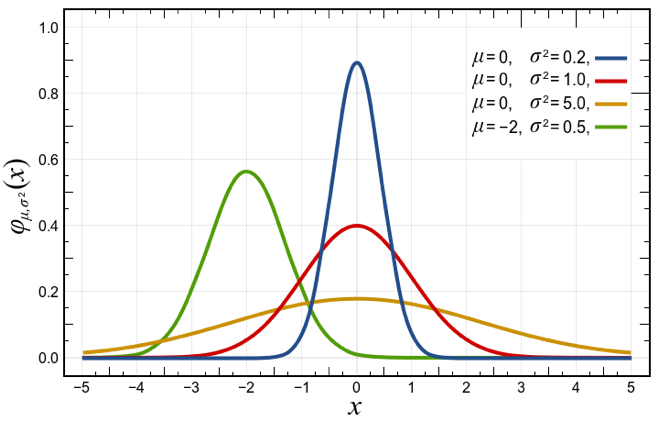
\includegraphics{./normal-distribution.png}
\caption{Normal Distribution \label{fig:normal-distribution}}
\end{figure}

If you use a \texttt{\textbackslash{}label\{fig:normal-distribution\}} in the figure caption, then you could use a

\texttt{\textbackslash{}ref\{fig:normal-distribution\}} to refer to this figure.
For example, please refer to Fig. \ref{fig:normal-distribution}.

\subsection{Footnote}\label{footnote}

In a paragraph, sometimes you need to make a further (but short) explanation for some keywords.
You could use footnotes to do this. The following are 2 footnotes examples.

The normal distribution is found by Carl Friedrich Gauss\footnote{Carl Friedrich Gauss (30 April 1777 -- 23 February 1855) was a German mathematician and physicist.}.

The student's t distribution is found by William Sealy Gosset\footnote{William Sealy Gosset (13 June 1876 -- 16 October 1937) was an English statistician.}.

\subsection{Assign index for keyworkds}\label{assign-index-for-keyworkds}

You can assign index for keyworks by using \texttt{Keywords\textbackslash{}index\{Keywords\}}.
The following are 2 examples.

The normal distribution is found by Carl Friedrich Gauss\index{Carl Friedrich Gauss}.

The student's t distribution is found by William Sealy Gosset\index{William Sealy Gosset}.

You can go to ``Index'' part in the last page to check if indexes are generated.

\subsection{Cite from bibliography/references}\label{cite-from-bibliographyreferences}

You have to define bibliography in the \texttt{yaml} header of the \texttt{md} first and then you can use \texttt{\textbackslash{}cite} to refer to it.
The following is a paragraph with 3 items cited.

This paragraph is an example of \textbf{\texttt{thebibliography}} environment using
in bibliography management. Three items are cited: \emph{The \LaTeX Companion}
book \cite{latexcompanion}, the Einstein journal paper \cite{einstein}, and the
Donald Knuth's website \cite{knuthwebsite}. The \LaTeX related items are
\cite{latexcompanion,knuthwebsite}.

\clearpage

\section{Math Equations}\label{math-equations}

The following are 2 examples for equations.

\subsection{Normal distribution}\label{normal-distribution}

The normal distribution is a continuous probability distribution with probability density function (pdf) defined as

\begin{equation}\label{eqn:normal-distribution}
f(x ; \mu, \sigma^{2}) = \frac{1}{\sqrt{2\pi\sigma^{2}}}e^{-\frac{\displaystyle (x - \mu)^{2}}{\displaystyle 2\sigma^{2}}}, \quad -\infty < x < \infty
\end{equation}

where

\begin{itemize}
\tightlist
\item
  \(\mu\) is the mean or expectation of the distribution.
\item
  \(\sigma\) is the standard deviation of the distribution.
\item
  \(\sigma^{2}\) is the variance of the distribution.
\end{itemize}

If you use a \texttt{\textbackslash{}label\{eqn:normal-distribution\}} in this equation, then you could use a

\texttt{\textbackslash{}ref\{eqn:normal-distribution\}} to refer to this equation.
For example, please refer to Eq. \ref{eqn:normal-distribution}.

\subsection{\texorpdfstring{\(t\)-distribution}{t-distribution}}\label{t-distribution}

The \(t\)-distribution is a continuous probability distribution with probability density function defined as

\begin{equation}\label{eqn:student-t}
f(x ; \nu) = \frac{\Gamma(\frac{\nu+1}{2})}{\sqrt{\nu\pi}\Gamma(\frac{\nu}{2})}
\left( 1 + \frac{x^{2}}{\nu} \right)^{\displaystyle -\frac{\nu+1}{\displaystyle 2}}
, \quad -\infty < x < \infty
\end{equation}

where

\begin{itemize}
\tightlist
\item
  \(\nu\) is the degrees of freedom and is a positive integer.
\item
  \(\Gamma\) is the gamma function.
\end{itemize}

If you use a \texttt{\textbackslash{}label\{eqn:student-t\}} in this equation, then you could use a

\texttt{\textbackslash{}ref\{eqn:student-t\}} to refer to this equation.
For example, please refer to Eq. \ref{eqn:student-t}.

\section{Advance Math for Align, Theorems and Proofs}\label{advance-math-for-align-theorems-and-proofs}

Examples in this section/chapter needs
the following option turned on in the \texttt{yaml} header of \texttt{md}

\begin{verbatim}
---
enable-adv-math-packages: true
.
.
.
...
\end{verbatim}

\subsection{Multi-line equation which aligns to the equal sign}\label{multi-line-equation-which-aligns-to-the-equal-sign}

\begin{align}
dP &= \frac{e^{-Q/2}}{(2\pi)^{k/2}}\frac{2\pi^{k/2}}{\Gamma(\frac{k}{2})}Q^{(k-1)/2}\frac{dQ}{2Q^{1/2}} \nonumber \\
   &= \frac{1}{2^{k/2}\Gamma(k/2)}Q^{k/2 - 1}e^{-Q/2}dQ \label{align:multi-line-eq-2nd} \\
   &= f(Q)dQ \label{align:multi-line-eq-3rd}
\end{align}

You can refer to one of its formula after the equal sign like this =\textgreater{} Eq. \ref{align:multi-line-eq-2nd}

\subsection{Theorem}\label{theorem}

\begin{theorem}\label{thm:X-2-chi}
If a random variable $Y = X^{2}$ where $X \sim N(0,1)$,
then $Y  \sim \chi^{2}_{1}$.
\end{theorem}

You can refer to this theorem like this =\textgreater{} Theorem \ref{thm:X-2-chi}

\subsection{Proof}\label{proof}

\begin{proof}\label{prf:X-2-chi}
Let $P(Y)$ be the cumulative distribution function of the random variable $Y$, then \\
for $y < 0$, $P(Y < y) = 0$ (since $Y = X^{2} \geq 0$ for all X) \\
for $y > 0$:
\begin{align}
P(Y < y) &= P(X^{2} < y) = P(|X| < \sqrt{y}) = P(-\sqrt{y} < X < \sqrt{y} \nonumber \\
         &= F_{x}(\sqrt{y}) - F_{x}(-\sqrt{y}) = F_{x}(\sqrt{y}) - (1 - F_{x}(\sqrt{y})) \nonumber \\
         & = 2F_{x}(\sqrt{y}) - 1 \nonumber \\
f_{Y}(y) &= 2\frac{d}{dy}F_{x}(\sqrt{y}) - 0 = 2\frac{d}{dy}(\int^{\sqrt{y}}_{-\infty}\frac{1}{\sqrt{2\pi}}e^{\frac{-t^{2}}{2}}dt) \nonumber \\
         &= 2\frac{1}{\sqrt{2\pi}}e^{-\frac{y}{2}}\frac{d}{dy}(\sqrt{y}) = 2\frac{1}{\sqrt{2}\sqrt{\pi}}e^{-\frac{y}{2}}(\frac{1}{2}y^{-\frac{1}{2}}) \nonumber \\
         &= \frac{1}{2^{\frac{1}{2}}\Gamma(\frac{1}{2})}y^{-\frac{1}{2}}e^{-\frac{y}{2}} \label{align:chi1-final}
\end{align}
where $F$ and $f$ are the cdf and pdf of the corresponding random variables. \\
Eq. \ref{align:chi1-final} is just the pdf of $\chi^{2}_{1}$-distribution, then we have proved that $Y  \sim \chi^{2}_{1}$.
\end{proof}

You can refer to this proof like this =\textgreater{} Proof \ref{prf:X-2-chi}

\renewcommand\refname{References}
\begin{thebibliography}{9}\label{thebibliography}
\addcontentsline{toc}{section}{References}

\bibitem{latexcompanion}
Michel Goossens, Frank Mittelbach, and Alexander Samarin. \emph{The \LaTeX Companion}. Addison-Wesley, Reading, Massachusetts, 1993.

\bibitem{einstein}
Albert Einstein. \emph{Zur Elektrodynamik bewegter Körper}. (German) {[}\emph{On the electrodynamics of moving bodies}{]}. Annalen der Physik, 322(10): 891--921, 1905.

\bibitem{knuthwebsite}
Knuth: Computers and Typesetting, \newline \texttt{http://www-cs-faculty.stanford.edu/\textasciitilde{}uno/abcde.html}

\end{thebibliography}

\printindex
\end{document}
